\documentclass[10pt,titlepage]{jsarticle}
%
%	和文: jsarticle, 欧文: article
%	titlepage: タイトルを独立したページにする.
%

\usepackage{
	amssymb,
	amsmath,
	amsthm,
	ascmac,
	mathrsfs,
	framed,
	color,
	bm,
	stmaryrd,
	clock,
}
%
%	amssymb, amsmath: 数学記号.
%	amsthm: 定理環境(\newtheorem).
%	ascmac: 文章を囲むscreen環境(screen, itembox, shadebox, etc. ).
%	mathrsfs: 花文字.
%	framed: leftbar環境.
%	color: 文字色の変更.
%	bm: 太文字.
%	stmaryrd: \longmapsfrom等.
%	clock: 時計.
%

\usepackage[dvipdfmx]{graphicx}
%
%	図の挿入.
%

\allowdisplaybreaks[4]
%
%	align環境において式の途中で改ページを許す.
%

\usepackage{indentfirst}
%
%	段落変更時に字下げをする.
%

\usepackage[dvipdfmx]{hyperref}
\usepackage{pxjahyper}
\hypersetup{colorlinks=true,urlcolor=blue,citecolor=blue,linkcolor=blue}
%
%	引用する際にリンクを付ける.
%

\usepackage[margin=15truemm]{geometry}
\usepackage{layout}
%
%	レイアウト. 例えば以下を参考.
%	https://dayinthelife.at.webry.info/201401/article_2.html
%

\usepackage[all]{xy}
\def\objectstyle{\displaystyle}
%
%	可換図式等を簡単に綺麗に書くことができる.
%	しかし蛇の補題等の複雑な図式には向かない. 例えば以下を参考.
%	http://www.math.u-ryukyu.ac.jp/~tsukuda/computer/tex/files/xypic-example.pdf
%	
%

\usepackage{tikz}
\usetikzlibrary{cd}
%
%	(たぶん)上のxyパッケージの上位互換. 蛇の補題等も書ける. ただし書き方が複雑.
%	http://alg-d.com/math/kan_extension/tikz.html
%	http://abenori.blogspot.com/2015/07/tikz-cd.html
%

\usepackage{mathtools}
\mathtoolsset{showonlyrefs,showmanualtags}
%
%	式を引用するときだけ式番号を表示.
%	これがあれば(align*とalignを混在させずに)align環境だけで済む.
%

\usepackage{listings}
\lstset{
	basicstyle={\ttfamily},
	identifierstyle={\small},
	commentstyle={\smallitshape},
	keywordstyle={\small\bfseries},
	ndkeywordstyle={\small},
	stringstyle={\small\ttfamily},
	frame={tb},
	breaklines=true,
	columns=[l]{fullflexible},
	numbers=left,
	xrightmargin=0zw,
	xleftmargin=3zw,
	numberstyle={\scriptsize},
	stepnumber=1,
	numbersep=1zw,
	lineskip=-0.5ex
}
%
%	プログラムのコードを載せる用. \begin{lstlisting}で書ける. 以下から拝借させていただいた.
% 	https://qiita.com/ta_b0_/items/2619d5927492edbb5b03
%

\theoremstyle{definition}
\newtheorem{thm}{定理}[section]
\newtheorem{prop}[thm]{命題}
\newtheorem{cor}[thm]{系}
\newtheorem{lem}[thm]{補題}
\newtheorem{defi}[thm]{定義}
\newtheorem{ex}[thm]{例}
\newtheorem{rem}[thm]{注意}
%
%	定理環境.
%	

\makeatletter
\newcommand{\MyMathOperators}[1]{\@for\op:=#1\do{
	\expandafter\edef\csname\op\endcsname{\noexpand\mathop{\noexpand\mathrm{\op}}\nolimits}
}}
\makeatother
\MyMathOperators{%
	Ker,%
	Coker,%
	Hom,%
	End,%
	Aut,%
	id,%
	Gal,%
	ch,%
	ord,%
	Spec,%
	Specm,%
	Frac,%
	rank,%
	corank,%
	sgn,%
	alg,%
	Reg,%
	Sel,%
}
\let\Re\relax
\DeclareMathOperator{\Re}{Re}
\let\Im\relax
\DeclareMathOperator{\Im}{Im}
\let\epsilon\relax
\DeclareMathOperator{\epsilon}{\varepsilon}
%
%	新しい数学演算子の定義. 例えば以下を参考.
%	https://mathlandscape.com/declaremathoperator/
%

\makeatletter
\newcommand{\MyAlphabet}[1]{\@tfor\Ch@r:=#1\do{
	\expandafter\edef\csname bb\Ch@r\endcsname{\noexpand\mathbb{\Ch@r}}
	\expandafter\edef\csname cal\Ch@r\endcsname{\noexpand\mathcal{\Ch@r}}
	\expandafter\edef\csname frak\Ch@r\endcsname{\noexpand\mathfrak{\Ch@r}}
	\expandafter\edef\csname scr\Ch@r\endcsname{\noexpand\mathscr{\Ch@r}}
}}
\makeatother
\MyAlphabet{ABCDEFGHIJKLMNOPQRSTUVWXYZabcdefghijklmnopqrstuvwxyz}
\newcommand{\ilim}[1][]{\mathop{\varinjlim}\limits_{#1}}
\newcommand{\plim}[1][]{\mathop{\varprojlim}\limits_{#1}}
\renewcommand{\bar}[1]{\overline{#1}}
\renewcommand{\tilde}[1]{\widetilde{#1}}
\renewcommand{\hat}[1]{\widehat{#1}}
%
%	新しい関数の定義.
%

\DeclarePairedDelimiter{\skakko}{\lparen}{\rparen} %括弧( )
\DeclarePairedDelimiter{\mkakko}{\lbrace}{\rbrace} %括弧{ }
\DeclarePairedDelimiter{\lkakko}{\lbrack}{\rbrack} %括弧[ ]
\DeclarePairedDelimiter{\gkakko}{\langle}{\rangle} %括弧< >
\DeclarePairedDelimiter{\abs}{\lvert}{\rvert} %絶対値| |
\DeclarePairedDelimiterX{\set}[2]{\lbrace}{\rbrace}{#1\,\delimsize\vert\,#2} %集合{ }
%
%	括弧の大きさ等を自動的に調整. 例えば以下を参考.
%	https://mathlandscape.com/declarepaireddelimiter/
%

\usepackage{lmodern}
\usepackage[T1]{fontenc}
\usepackage{bxjalipsum}
\usepackage[leftmarker]{mindflow}
\renewcommand{\mindflowTextFont}{\normalfont\footnotesize\sffamily\itshape}
\renewcommand{\mindflowNumFont}{\normalfont\footnotesize\sffamily}
\renewcommand{\mindflowLeft}{\hspace{1em}\(\succ\)}
\renewcommand{\mindflowRight}{\(\prec\)}
\setlength{\mindflowLineHeight}{1pt}
%
%	メインテキスト中にアイデア, 注釈, 計画を書けるパッケージ. 例えば以下を参考.
%	https://konoyonohana.blog.fc2.com/blog-entry-608.html
%	\begin{mindflow} \end{mindflow}と使用.
%

\newenvironment{gyoukan}{\begin{leftbar}\color{gray}}{\color{black}\end{leftbar}}
%
%   行間を書く用.
%

\usepackage[OT2,T1]{fontenc}
\DeclareSymbolFont{cyrletters}{OT2}{wncyr}{m}{n}
\DeclareMathSymbol{\Sha}{\mathalpha}{cyrletters}{"58}
%
%	キリル文字, 特にShaを表示させる用.
%

\renewcommand{\theenumi}{\roman{enumi}}
\renewcommand{\labelenumi}{(\theenumi)}
\renewcommand{\theenumii}{\theenumi-\alph{enumii}}
\renewcommand{\labelenumii}{(\theenumii)}
%
%	enumerate環境の見出し変更. 例えば以下を参考.
%	https://mathlandscape.com/latex-enum/
%

\def\MyName{name} % 変更
\def\MyMailAddress{mail address} % 変更
\title{title} % 変更
\author{\MyName \thanks{mail: \href{\MyMailAddress}{\texttt{\MyMailAddress}}}}
\date{最終更新: \today \texthours 時 \textminutes 分 \clocktime}
%
%	タイトルに表示する情報.
%

\begin{document}
\maketitle
\tableofcontents
\newpage
%
%	タイトル及び目次の表示.
%

%%%%% 本文 %%%%%

\section{記号}

\subsection{数学文字}

黒板太字(mathbb)は
\begin{align}
	\bbA, \bbB, \bbC, \bbD, \dots
\end{align}
のように書くことができる. 筆記体(mathcal)は
\begin{align}
	\calA, \calB, \calC, \calD, \dots
\end{align}
のように書くことができる. フラクトゥール(mathfrak)は
\begin{align}
	\frakA, \frakB, \frakC, \frakD, \dots, \fraka, \frakb, \frakc, \frakd, \dots
\end{align}
のように書くことができる. 花文字(mathscr)は
\begin{align}
	\scrA, \scrB, \scrC, \scrD, \dots
\end{align}
のように書くことができる.

\subsection{数学作用素}
プリアンブルの\verb|\MyMathOperators|に登録した文字は数学作用素として書くことができる.
例えば
\begin{align}
	\Ker f, \ \Hom(\frakg, \frakh), \ \Gal(\bar{K}/K), \ \Spec A, \ \rank E(\bbQ), \ \Sel^{(\phi)}(E/K)
\end{align}
のように使用可能.

\section{数式}

align環境で数式を書く際には, ラベリングをするかどうかに関わらず「*」は付けなくてよい.
例えば以下の数式
\begin{align}
	\zeta(s)\coloneqq\sum_{n=1}^{\infty}\frac{1}{n^s} \label{eq:RiemannZetaFunction}
\end{align}
は引用していないので, 式番号は付いていない. しかし
\begin{align}
	f(z_0)=\frac{1}{2\pi i}\oint_{C}\frac{f(z)}{z-z_0}dz \label{eq:CauchyIntegralFormula}
\end{align}
は式\eqref{eq:CauchyIntegralFormula}と引用したので式番号が表示されている.
括弧のサイズを調整する際は本来\verb|\left( \right)|, \verb|\left\{ \right\}|, \verb|\left[ \right]|と記述するが
\begin{align}
	\skakko*{\frac{q}{p}}, \ \mkakko*{0, \frac{k}{m}}, \ \lkakko*{\frac{1}{n+1}x^{n+1}}_{x=a}^{b}
\end{align}
のように書くことができる.

\section{定理・コメント}

\subsection{定理環境}

定義や命題等は, 以下のようにして記述する:
\begin{defi}[群]\label{defi:Group}
	空でない集合$G$が\textbf{群}であるとは, 写像
	\begin{align}
		\phi: G\times G\to G
	\end{align}
	で以下の三つの条件を満たすものが存在することをいう.
	\begin{description}
		\item[結合法則] ${}^{\forall} g, h, i\in G, \ \phi(\phi(g, h), i)=\phi(g, \phi(h, i))$.
		\item[単位元] ${}^{\exists} e\in G \ \text{s.t.} \ {}^{\forall} g\in G, \ \phi(g, e)=\phi(e, g)=e$.
		\item[逆元] ${}^{\forall} g\in G, {}^{\exists} g^{-1}\in G \ \text{s.t.} \ \phi(g, g^{-1})=\phi(g^{-1}, g)=e$. 
	\end{description}
	$\phi(g, h)$のことを単に, $g\cdot h$や$gh$と書くことがある.
\end{defi}

\begin{prop}[単位元の一意性]\label{prop:UniqueIdentityElement}
	群$G$の単位元$e$は一意的に存在する.
\end{prop}
\begin{proof}
	$e, e'\in G$を単位元とする. Definition \ref{defi:Group}より
	\begin{align}
		e
		&=e\cdot e' \quad (\because e'\text{は単位元})\\
		&=e' \quad (\because e\text{は単位元})
	\end{align}
	が成り立つ. したがって群の単位元は一意的に存在する.
\end{proof}

\begin{rem}\label{rem:UniqueInverseElement}
	Proposition \ref{prop:UniqueIdentityElement}と同様にして, 逆元の一意性も証明することができる.
\end{rem}

\subsection{コメント}

証明のアイデアを書く際は, 本文や証明のスペースと混同しないように以下の環境で書くことが可能である.
\begin{mindflow}
	Proposition \ref{prop:UniqueIdentityElement}の証明は, 以下のようなアイデアで示すことができる.
	まず単位元の一意性を証明する際は, 単位元が$e, e'$と二つ存在することを仮定し
	\begin{align}
		e=e'
	\end{align}
	を示すのが定石である. また, 使える道具としては単位元の性質くらいしか知らない状態であることを踏まえると
	上のような証明方法になるだろう.
\end{mindflow}
また, TeXで数学書の写経を行う際等に, 行間の証明のために新たに定理環境を使用するのは避けたい, という場合がある.
そのような場合は, 以下の環境で書くことが可能である.
\begin{gyoukan}
	Definition \ref{defi:Group}における群の定義は少し修正する必要がある.
	それは, 逆元の公理に単位元が含まれていることが理由である.
	つまり, 単位元と逆元の公理を合わせて
	\begin{align}
		{}^{\exists}e\in G \ \text{s.t.} \ {}^{\forall}g\in G, [g\cdot e=e\cdot g=g \ \wedge \ {}^{\exists} g^{-1}\in G \ \text{s.t.} \ g\cdot g^{-1}=g^{-1}\cdot g=e]
	\end{align}
	と書くのが正しい.
\end{gyoukan}

\section{図}

\subsection{XY-pic}

準同型定理の図式は以下のようにして書ける.
\begin{align}
	\xymatrix{
		G \ar[r]^-{f} \ar[d]_-{\pi} & \Im f \\
		G/\Ker f \ar@{.>}[ur]_-{\simeq} & \ar@{}[lu]|(.65){\circlearrowright} 
	}
\end{align}
ファイバー積の普遍性は以下のようにして書ける.
\begin{align}
	\xymatrix{
		T \ar@/^10pt/[rrd]^-{t} \ar@/_10pt/[ddr]_-{s} \ar@{.>}[rd]^-{{}^{\exists!}u}& & \\
		 & X\times_{Z}Y \ar[r]^-{q} \ar[d]_-{p} & Y \ar[d]^-{g} \\
		 & X \ar[r]_-{f} & Z
	}
\end{align}

\subsection{TikZ}

準同型定理の図式は以下のようにして書ける.
\begin{align}
	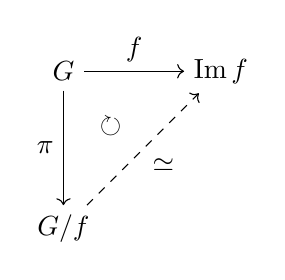
\begin{tikzpicture}[auto]
		\node (G) at (0, 2) {$G$};
		\node (Imf) at (2, 2) {$\Im f$};
		\node (GKerf) at (0, 0) {$G/\Ker f$};
		\node (Circle) at (0.6, 1.3) {$\circlearrowright$};
		\draw[->] (G) to node {$f$} (Imf);
		\draw[->] (G) to node[swap] {$\pi$} (GKerf);
		\draw[->, dashed] (GKerf) to node[swap] {$\simeq$} (Imf);
	\end{tikzpicture}
\end{align}
ファイバー積の普遍性は以下のようにして書ける.
\begin{align}
	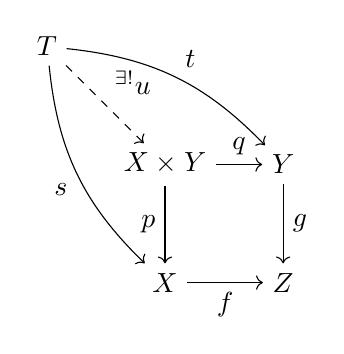
\begin{tikzpicture}[auto]
		\node (T) at (0, 3) {$T$};
		\node (X) at (1.5, 0) {$X$};
		\node (XxY) at (1.5, 1.5) {$X\times_{\bbZ}Y$};
		\node (Z) at (3, 0) {$Z$};
		\node (Y) at (3, 1.5) {$Y$};
		\draw[->, dashed] (T) to node {${}^{\exists!}u$} (XxY);
		\draw[->] (T) to[bend left=20] node {$t$} (Y);
		\draw[->] (T) to[bend right=20] node[swap] {$s$} (X);
		\draw[->] (XxY) to node {$q$} (Y);
		\draw[->] (XxY) to node[swap] {$p$} (X);
		\draw[->] (Y) to node {$g$} (Z);
		\draw[->] (X) to node[swap] {$f$} (Z);
	\end{tikzpicture}
\end{align}

\section{アルゴリズム・コード}




%%%%%%%%%%%%%%%%

\bibliographystyle{plain}
\bibliography{bibs}
%
%	bibtexによる参考文献の表示.
%	bibs.bibというbibファイルを作り, そこに文献データを登録しておく.
%	引用文献を表示させるには
%	「LaTeX」で1回タイプセット -> 「BibTeX」で1回タイプセット -> 「LaTeX」で3回タイプセット
%	とする. それ以降はbibファイルに加除がないなら「BibTeX」によるタイプセットは必要なし.
%	plain(jplain)は参考文献をアルファベット順で出力. unsrt(junsrt)は引用された順で出力する.
%	ただしlatexmkを使用したタイプセットならば上で述べた複数回のタイプセットは自動的に一度でやってくれる.
\end{document}